\documentclass[10pt,a4paper]{article}
\usepackage[utf8]{inputenc}
\usepackage[italian]{babel}
\usepackage{amsmath}
\usepackage{amsfonts}
\usepackage{amssymb}
\usepackage{graphicx}
\usepackage[left=2cm,right=2cm,top=2cm,bottom=2cm]{geometry}
\newcommand{\rem}[1]{[\emph{#1}]}

\author{Gruppo BN \\ Federico Belliardo, Marco Costa, Lisa Bedini}
\title{Esperienza sull'effetto fotoelettrico}
\begin{document}

\maketitle
\section{Scopo dell'esperienza}
Obiettivo dell'esperienza è la verifica dell'effetto fotoelettrico, e la stima della grandezza del fattore $h/e$, dove $h$ \'e la costante di Planck e $e$ la carica dell'elettrone.\\
%forse mettere la fomrletta E = h\nu?
\section{Materiale occorrente}
\begin{itemize}
\item Lampada a LED;
\item Tubo fotomoltiplicatore Philips XP2412 B;
\item Filtri interferenziali (Balzers e Newport);
\item Scatola nera
\item Generatore di tensione continua;
\item Multimetro digitale;
\item Picoamperometro digitale;
\end{itemize}
\section{Descrizione esperimento}

Si è montato il circuito in figura \ref{circuito}. Nella scatola nera erano fissati il fotomoltiplicatore e la lampada a LED che serviva da sorgente luminosa. Durante l'esperienza, abbiamo posizionato i filtri nell'apposito supporto, avendo cura che fossero ortogonali al piano di appoggio della scatola e quindi al fascio luminoso.

Per ogni filtro si è misurata la corrente in funzione del potenziale applicato ai capi del fotomoltiplicatore. Per un certo potenziale $V_0$ (detto di azzeramento) la corrente di elettroni (estratti per effetto fotoelettrico) che arriva all'amperometro si annulla. Questo ci consente di stimare la massima energia cinetica degli elettroni come $eV_0$, da confrontare con l'energia dei fotoni incidenti $E_{\gamma}=hf$. 
 Il modello teorico prevede che valga la relazione
 \begin{equation}\label{eq:fotoelettrico}
 eV_0 = hf + W
 \end{equation}, con $f$ frequenza del fotone incidente e $W$ lavoro di estrazione del metallo. Una volta noti i potenziali di azzeramento in funzione delle frequenze eseguiamo un fit per verificare la relazione \ref{eq:fotoelettrico}.
\begin{figure}[!htb]
  \centering
  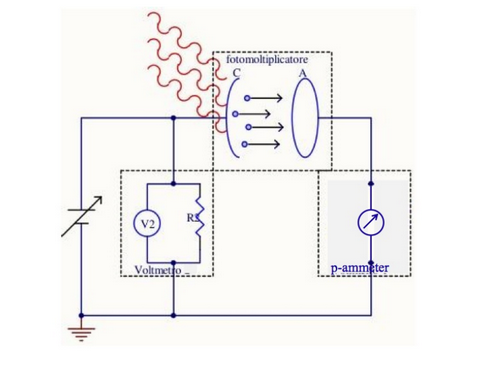
\includegraphics[scale=1.0]{circuito.png}
\caption{Schema circuito dell'esperimento e di acquisizione dati.\label{circuito}}
\end{figure}


\section{Misure}

Per ogni filtro abbiamo acquisito dalle quindici alle venti misure di tensione ai capi del tubo fotomoltiplicatore e della relativa corrente.
Abbiamo iniziato le acquisizioni da $V\simeq 0$ V e variato progressivamente il potenziale fino a che la corrente non raggiungeva un valore asintotico. Abbiamo posto particolare attenzione alla presa dati sia nella regione asintotica sia in quella in cui il grafico curvava significativamente: in questo modo è stato più facile estrarre i parametri nei fit dei punti successivi della relazione.
La tensione di frenamento è stata misurata tramite multimetro digitale. La corrente circolante nel circuito è stata misurata tramite picoamperometro.
La lettura della corrente veniva fatta dopo un tempo sufficientemente lungo da fare in modo che il valore riportato dallo strumento si fosse stabilizzato. %anche se non è stato sempre facile lo scriviamo nelle conclusioni?
Come errore sulle differenze di potenziale applicate si sono prese le incertezze riportate sul manuale del multimetro.
Come errore sulla misura di corrente si  presa l'ultima cifra "stabile" nella lettura, che si rivelava essere maggiore dell'incertezza strumentale riportata sul manuale del picoamperometro (0.4\% + 1 digit sulle scale usate) %(0.5\% + 1 digit per il voltmetro e 0.4\% + 1 digit e 0.2\% + 1 digit per il picoamperometro, rispettivamente sulle scale dei 20 nA e dei 200 nA
Per stimare le lunghezze d'onda dei filtri, e quindi della frequenza effettiva dei fotoni incidenti, abbiamo usato la tabella fornita (\ref{tab:filtri}).
L'incertezza associata ad ogni lunghezza d'onda riportata è stata presa come metà della FWHM della banda passante riportata sul data sheet per i filtri Newport, mentre per i Balzers si è assunto un valore del $2\%$ di incertezza. 

\begin{table}[!htb]
\begin{center}
\begin{tabular}{|c|c|c|}
\hline 
Colore & $\lambda$ (nm) & Tipo \\ 
\hline 
Arancione & $602\pm  12$  & Balzers\\ 
\hline 
Giallo & $577\pm 11$ & Newport\\ 
\hline 
Verde & $546\pm 10$ & Balzers\\ 
\hline 
Verde-azzurro & $499 \pm 11$ & Newport\\ 
\hline 
Azzurro & $ 450\pm 10$ & Balzers \\ 
\hline
Blu & $405\pm 11 $ & Newport\\ 
\hline
\end{tabular} 
\caption{Caratteristiche dei filtri utilizzati. \label{tab:filtri}}
\end{center}
\end{table}

Di seguito sono riportate le tabelle dei dati raccolti per ogni filtro. %immagino che vadano messe?
\\

\begin{table}[!htb]\centering
\begin{tabular}{|c|c|c|c|}
\hline
$V$ (mV) & $\sigma V$ (mV) & $I$ (nA) & $\sigma I$ (nA)\\
\hline
9.6 & 0.1 & 15.57 & 0.05\\
69.5 & 0.4 & 10.36 & 0.05\\
119.9 & 0.7 & 7.11 & 0.05\\
171 & 1 & 4.67 & 0.05\\
229 & 2 & 2.67 & 0.05\\
276 & 2 & 1.57 & 0.05\\
322 & 3 & 0.72 & 0.05\\
371 & 3 & 0.07 & 0.05\\
526 & 4 & -1.11 & 0.05\\
618 & 4 & -1.40 & 0.05\\
913 & 6 & -1.67 & 0.05\\
1424 & 8 & -1.74 & 0.01\\
1606 & 9 & -1.76 & 0.01\\
1920 & 10 & -1.78 & 0.01\\
\hline
\end{tabular}
\caption{Dati filtro Arancio.}
\end{table}


\begin{table}[!htb]\centering
\begin{tabular}{|c|c|c|c|}
\hline
$V$ (mV) & $\sigma V$ (mV) & $I$ (nA) & $\sigma I$ (nA)\\
\hline
11.4 & 0.2 & 11.8 & 0.1\\
49.1 & 0.3 & 8.52 & 0.01\\
109.0 & 0.6 & 3.76 & 0.01\\
164.0 & 0.9 & 2.40 & 0.01\\
201 & 1 & 1.35 & 0.05\\
250 & 2 & 0.16 & 0.01\\
304 & 2 & -0.90 & 0.01\\
352 & 3 & -1.18 & 0.01\\
456 & 3 & -1.78 & 0.01\\
503 & 4 & -1.90 & 0.01\\
553 & 4 & -1.99 & 0.01\\
610 & 4 & -2.04 & 0.01\\
871 & 5 & -2.17 & 0.01\\
1230 & 7 & -2.23 & 0.01\\
1613 & 9 & -2.27 & 0.01\\
1940 & 10 & -2.30 & 0.01\\
2010 & 20 & -2.30 & 0.01\\
2300 & 20 & -2.32 & 0.01\\
\hline
\end{tabular}
\caption{Dati filtro Giallo.}
\end{table}

\begin{table}[!htb]\centering
\begin{tabular}{|c|c|c|c|}
\hline
$V$ (mV) & $\sigma V$ (mV) & $I$ (nA) & $\sigma I$ (nA)\\
\hline
9.9 & 0.1 & 17.42 & 0.01\\
71.1 & 0.5 & 10.3 & 0.1\\
141 & 2 & 5.40 & 0.05\\
220 & 2 & 1.84 & 0.05\\
300 & 3 & -0.14 & 0.05\\
404 & 3 & -1.33 & 0.05\\
452 & 3 & -1.76 & 0.05\\
503 & 4 & -1.91 & 0.05\\
551 & 4 & -1.98 & 0.05\\
802 & 5 & -2.07 & 0.05\\
1219 & 7 & -2.11 & 0.05\\
1563 & 9 & -2.13 & 0.05\\
1800 & 10 & -2.15 & 0.05\\
2090 & 20 & -2.16 & 0.05\\
2490 & 20 & -2.17 & 0.05\\
\hline
\end{tabular}
\caption{Dati filtro Verde.}
\end{table}

\begin{table}[!htb]\centering
\begin{tabular}{|c|c|c|c|}
\hline
$V$ (mV) & $\sigma V$ (mV) & $I$ (nA) & $\sigma I$ (nA)\\
\hline
10.2 & 0.2 & 6.18 & 0.01\\
71.7 & 0.5 & 4.13 & 0.01\\
122.7 & 0.7 & 2.85 & 0.05\\
180 & 1 & 1.73 & 0.02\\
347 & 3 & -0.33 & 0.05\\
404 & 3 & -0.68 & 0.02\\
451 & 3 & -0.91 & 0.01\\
508 & 4 & -1.12 & 0.01\\
551 & 4 & -1.23 & 0.01\\
601 & 4 & -1.32 & 0.01\\
885 & 5 & -1.45 & 0.01\\
1206 & 7 & -1.47 & 0.01\\
1608 & 9 & -1.49 & 0.01\\
2140 & 20 & -1.51 & 0.01\\
2570 & 20 & -1.52 & 0.01\\
\hline
\end{tabular}
\caption{Dati filtro Verde-Azzurro.}
\end{table}


\begin{table}[!htb]\centering
\begin{tabular}{|c|c|c|c|}
\hline
$V$ (mV) & $\sigma V$ (mV) & $I$ (nA) & $\sigma I$ (nA)\\
\hline
10.4 & 0.2 & 10.36 & 0.05\\
71.6 & 0.5 & 7.49 & 0.01\\
137.6 & 0.8 & 5.10 & 0.01\\
201 & 2 & 3.32 & 0.01\\
304 & 3 & 1.24 & 0.05\\
404 & 3 & 0.02 & 0.05\\
504 & 4 & -0.94 & 0.02\\
552 & 4 & -1.38 & 0.01\\
601 & 4 & -1.62 & 0.01\\
647 & 4 & -1.80 & 0.01\\
701 & 5 & -1.96 & 0.01\\
752 & 5 & -2.07 & 0.01\\
951 & 6 & -2.26 & 0.01\\
1207 & 7 & -2.29 & 0.01\\
1498 & 8 & -2.31 & 0.01\\
1702 & 10 & -2.33 & 0.01\\
2220 & 20 & -2.35 & 0.01\\
\hline
\end{tabular}
\caption{Dati filtro Azzurro.}
\end{table}


\begin{table}[!htb]\centering
\begin{tabular}{|c|c|c|c|}
\hline
$V$ (mV) & $\sigma V$ (mV) & $I$ (nA) & $\sigma I$ (nA)\\
\hline
10.3 & 0.2 & 1.71 & 0.01\\
53.3 & 0.4 & 1.36 & 0.01\\
98.4 & 0.6 & 1.05 & 0.02\\
148.4 & 0.8 & 0.77 & 0.02\\
200 & 2 & 0.53 & 0.02\\
319 & 3 & 0.14 & 0.03\\
379 & 3 & 0.02 & 0.02\\
468 & 3 & -0.117 & 0.002\\
510 & 4 & -0.145 & 0.002\\
564 & 4 & -0.188 & 0.002\\
625 & 4 & -0.212 & 0.002\\
684 & 4 & -0.230 & 0.001\\
805 & 5 & -0.249 & 0.001\\
1133 & 7 & -0.262 & 0.001\\
1509 & 9 & -0.267 & 0.002\\
1705 & 10 & -0.269 & 0.002\\
2270 & 20 & -0.273 & 0.002\\
\hline
\end{tabular}
\caption{Dati filtro Blu.}
\end{table}

\section{Elaborazione dati: stima potenziale di azzeramento $V_0$}
Per stimare il potenziale di azzeramento relativo ad una data frequenza dei fotoni incidenti abbiamo percorso i seguenti due metodi.
\subsection{Metodo A}
Per ogni filtro si stima la corrente di emissione dall'anodo $I_A$. In prima approssimazione, si suppone che questa non dipenda significativamente dal potenziale di frenamento applicato. Pertanto si assume che la fotocorrente catodica $I_{C}$ sia $I-I_A$. 
Dati gli andamenti della corrente, si esegue un fit con la funzione modello $\sqrt(I_C)=aV +b$. Per il fit si è utilizzata la funzione \emph{curvefit} della libreria \emph{pylab} con l'opzione \emph{$absolute\,sigma = "false"$}, perché il modello di fit usato non è realistico.
Una volta estratti i parametri, si trova il potenziale di azzeramento $V_0$ ponendo 
\begin{equation}\label{eq:v0parabola}
I_{C}=0\rightarrow V_0=-b/a
\end{equation}
Per stimare la corrente di emissione dell'anodo, si sono considerati i dati in regime asintotico e si è eseguito un fit con funzione modello $y = b$.
(Dati i cui valori di corrente differiscono dal valore di corrente massimo per meno del $5\%$ vengono considerati asintotici).
In tabella \ref{tab:asintotico} si sono riportati i parametri di fit.

\begin{table}[!htb]
\centering
\begin{tabular}{|c|c|c|}
\hline
Colore & $b$ (nA) & $\chi ^2 $/ndof\\
\hline
Arancio & $-1.8\pm0.1$ & 11.2/3\\
\hline
Giallo & $-2.3\pm 0.1$ & 157.0/5\\
\hline
Verde & $-2.1\pm 0.1$ & 0.9/4\\
\hline
Verde-Azzurro & $-1.49\pm 0.05$ & 32.2/4\\
\hline
Azzurro & $-2.3 \pm 0.1$ & 49.1/4\\
\hline
Blu & $-0.27\pm0.01$ & 29.9/3\\
\hline
\end{tabular}
\caption{Risultati fit del regime asintotico.\label{tab:asintotico}}
\end{table}

Si osserva che i valori della corrente hanno una debole dipendenza dal potenziale: tendono infatti a crescere in valore assoluto all'aumentare di $V$.
In effetti l'ipotesi che la corrente anodica non dipenda dal potenziale applicato non è confermata dal $\chi ^2$.
Ai fini dei fit abbiamo ritenuto sensato considerare come corrente asintotica il valor medio sui punti presi.
Come incertezza abbiamo preso la semidispersione dei valori di corrente dalla media. Una volta ottenuto il valore della corrente asintotica, è stato eseguito un fit con la funzione modello parabolica sui dati, escludendo quelli in regime asintotico (che non possono rispettare un simile andamento).
I risultati dei fit sono riportati  nel grafico \ref{fig:fitparabolico}.
Nelle tabelle  \ref{tab:fitparabolico} si sono riportati i $\chi ^2$ e il relativo potenziale di arresto $V_0$ calcolato dai parametri tramite l'equazione \ref{eq:v0parabola}.

\begin{table}[!htb]
\centering
\begin{tabular}{|c|c|c|}
\hline
Colore & $\chi ^2$/ndof & $V_0$ (mV)\\
\hline
Arancio & 5358/8 & $470\pm 1$ \\
\hline
Giallo & 113247/10 & $477\pm 1$\\
\hline
Verde & 37815/8 & $ 552 \pm 1$\\
\hline
Verde-Azzurro & 18178/8 & $520\pm 1$\\
\hline
Azzurro & 60091/10 & $648\pm 1$\\
\hline
Blu & 220/11 & $658\pm 1$\\
\hline
\end{tabular}
\caption{$\chi^2$ e $V_0$ per il fit parabolico.\label{tab:fitparabolico}}
\end{table}


\begin{figure}[!htb]
\centering
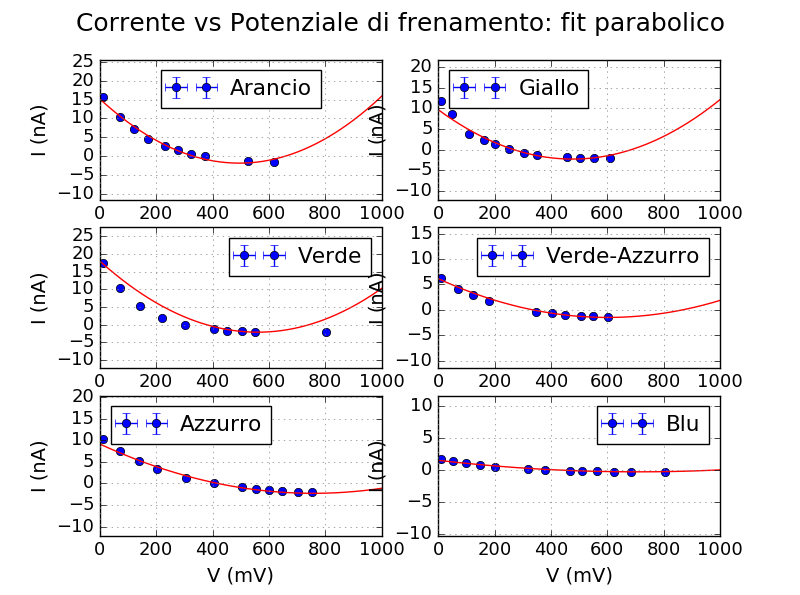
\includegraphics[scale=0.9]{fitparabolico.png}
\caption{Corrente in funzione del potenziale di frenamento per le varie frequenze (fit parabolico).\label{fig:fitparabolico}}
\end{figure}

L'errore su $V_0$ è stato calcolato propagando gli errori in quadratura dall'equazione \ref{eq:v0parabola}.
I $\chi ^2$ normalizzati sono dell'ordine delle migliaia : si evince che l'andamento non è affatto rispettato. Inoltre i potenziali di azzeramento estratti non sono in accordo con quanto predetto dal modello, nè con quanto ottenuto nel punto successivo. Pertanto  abbiamo continuato l'analisi senza eseguire il fit lineare con questi potenziali di azzeramento: non ci aspettiamo risultati coerenti con il modello e con il fit del prossimo punto.
\subsection{Metodo B}
Per ogni filtro si è stimato il relativo potenziale di azzeramento $V_0$ corrispondente alla tensione per cui la corrente fotocatodica risulta compatibile con 0 entro una incertezza $\delta I$. Per fare ciò si è eseguito un fit per ogni set di misure con la funzione modello
\begin{equation}\label{eq:fitexp}
I(V)=\bar{I}(e^{a(\bar{V}-V)}-1)
\end{equation}
Si osservi che con questa definizione $\bar(I)$ rappresenta il modulo della  corrente asintotica misurata.
I risultati dei fit sono riportati nella tabella \ref{tab:fitexp} e nel grafico \ref{fig:fitexp}.
\begin{table}[!htb]
\centering
\begin{tabular}{|c|c|c|c|c|}
\hline
Colore & $a$ $\mbox{mV}^{-1}$ &$\bar{V}$ (mV) & $\bar{I}$ (nA) & $\chi^2$/ndof\\
\hline
Arancio & $(6\pm 3)\cdot 10 ^{-3}$ & $380 \pm 1$ & $1.762\pm 0.07$ & 20/11\\
\hline
Giallo & $(7\pm 0.3) \cdot 10^{-3}$ & $248\pm 6$ & $2.23 \pm 0.07$ & 6100/15\\
\hline 
Verde & $(7 \pm 0.03)\cdot 10 ^ {-3}$ & $300 \pm 4$ & $2.23 \pm 0.05$ & 104/12 \\
\hline
Verde-Azzurro & $(5\pm 0.1)\cdot 10^{-3}$ & $304\pm 6$ & $1.55 \pm 0.04$ & 638 /12\\
\hline 
Azzurro & $(4 \pm 0.1)\cdot 10^{-3}$ & $384\pm 5$ & $2.43 \pm0.04$ & 1466/14\\
\hline
Blu & $(6\pm 0.09)\cdot 10^{-3} $ & $366\pm4$  &$0.273 \pm0.03$ & 195/14\\
\hline

\end{tabular}
\caption{Risultati dei fit con modello esponenziale.\label{tab:fitexp}}
\end{table}
\begin{figure}[!htb]
\centering
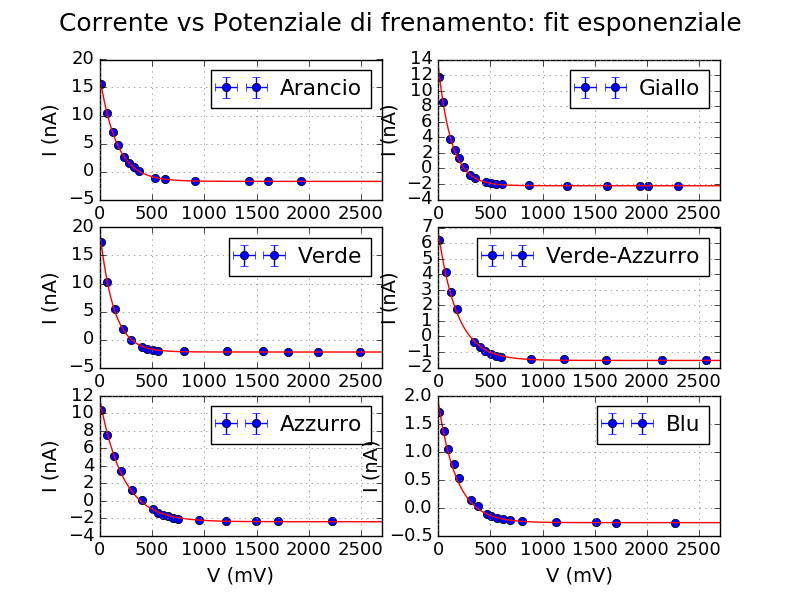
\includegraphics[scale=0.9]{fitesponenziale.png}
\caption{Grafici con le correnti misurate in funzione dei potenziali di frenamento per le varie frequenze (fit esponenziale).\label{fig:fitexp}}
\end{figure}

Anche per questo fit si è utilizzata la funzione \emph{curvefit} della libreria \emph{pylab} con l'opzione \emph{$absolute\,sigma = "false"$}.
I valori dei $\chi^2$ normalizzati vanno dalle decine alle centinaia: in effetti non ci si aspetta che l'andamento della funzione $I(V)$ sia davvero un esponenziale, ma semplicemente un andamento approssimativo con il quale estrarre dei parametri utili per i calcoli successivi.
Per ricavare $V_0$ è necessario risolvere l'equazione
\begin{equation}\label{eq:v0exp}
I(V_0)=-\bar{I}+\delta(I)\Rightarrow V_0=\bar{V}+\frac{1}{a}\ln\frac{\bar{I}}{\delta I}
\end{equation} 
Dobbiamo dunque stimare l'incertezza $\delta I$. 
Si osserva intanto che la corrente anodica non è davvero indipendente dalla differenza di potenziale applicato: guardando i dati si osserva che, anche per grandi $V$ il valore "asintotico" della corrente tende a crescere in valore assoluto.
Ai fini della stima abbiamo considerato l'errore estratto dal fit del parametro $\bar{I}$: anche se l'andamento complessivo della curva non sarà ben descritta da un esponenziale, è ragionevole supporre che la corrente anodica non sia perfettamente una costante ma tenda ad un valore limite esponenzialmente (almeno nella regione asintotica).
 
A questo scopo non abbiamo considerato nè l'errore dovuto alla stabilità (ossia quello effettivamente riportato sui dati), nè  l'errore strumentale (dell'ordine dello 0.4\% nelle scale usate) perchè più piccoli rispetto all'errore sui parametri.

Sebbene la scelta di $\delta I$ appaia arbitraria, questa non influisce sul fit lineare finale e sul valore del coefficiente angolare della retta $h/e$. Infatti, essendo sia il parametro $a$ che il valore dei $\delta I$ circa lo stesso per le varie frequenze utilizzate, i potenziali di azzeramento $V_0$ vengono traslati della stessa quantità se si varia $\delta I$ della stessa quantità per le varie frequenze.
In tabella \ref{tab:V_0} sono riportati i valori dei potenziali ottenuti in funzione del colore. Gli errori su $V_0$ estratti sono stati calcolati propagando in quadratura gli errori dei parametri (stimati dal fit) che compaiono in \ref{eq:v0exp}.
\begin{table}[!htb]
\centering
\begin{tabular}{|c|c|c|}
\hline
Colore & $\delta I$ (nA) & $V_{0}$(mV)\\
\hline
Arancio & 0.07 & $930\pm 10$\\
\hline
Giallo & 0.07 & $693 \pm 20$\\
\hline
Verde & 0.07 & $808 \pm 30$\\
\hline
Verde-Azzurro & 0.04 & $962\pm 30$ \\
\hline
Azzurro & 0.04 & $1290 \pm 30$\\
\hline
Blu & 0.03 & $790 \pm 10$\\
\hline
\end{tabular}
\caption{Valori del potenziale di azzeramento in funzione del filtro e del $\delta I$ usato.\label{tab:V_0}}
\end{table}
\section{Relazione frequenza-$V_0$}
Una volta ottenuti i potenziali di azzeramento per le varie frequenze, abbiamo eseguito un fit secondo la funzione modello $V_0=a\cdot f + b$.
Secondo il modello teorico $a = h/e\simeq 4.1 \mbox{V}\cdot\mbox{s}\cdot10^{-15}$.
Il risultato del fit è riportato in figura \ref{fig:fitfinale}.
\begin{figure}[!htb]
\centering
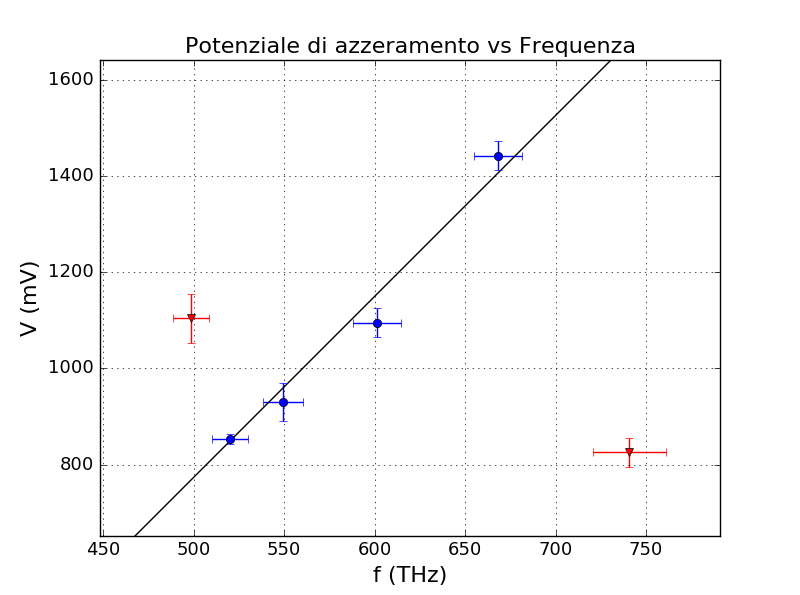
\includegraphics[scale=0.7]{fitfinale.png}
\caption{Grafico del potenziale di azzeramento in funzione della frequenza. I punti esclusi hanno colore e marker diversi.\label{fig:fitfinale}}
\end{figure}

Come valore del coefficiente angolare abbiamo ottenuto $a = (3.9\pm 0.2)\cdot10^{-15} \mbox{V}\cdot{s}$, in buon accordo con il valore atteso.
Si ha $\chi ^2$/ndof=0.8/2, il che indica che si siano sovrastimati gli errori.
Per il calcolo del $\chi^2$ si è considerato anche l'errore, non trascurabile, sulle frequenze, propagandolo con un valore stima di $3.5\cdot 10^{-15}\mbox{V}\cdot{s}$ per il coefficiente angolare.
Il $V_0$ per il filtro arancione non è in accordo con l'andamento teorico. In effetti a questa frequenza (più bassa delle altre), i fotoni hanno meno energia rispetto agli altri i casi. Il materiale eccitato nel fotomoltiplicatore è costituito da due tipi di metallo; solo uno di questi tuttavia riesce ad essere eccitato a queste energie. Pertanto il comportamento della corrente è  diverso rispetto agli altri.
Anche il potenziale di azzeramento per il filtro blu non è in accordo con quanto previsto, ma non siamo riusciti a trovare una spiegazione di tale fenomeno. Pertanto abbiamo escluso dal fit lineare i dati ricavati da questi filtri.
\section{Corrente anodica}
Successivamente abbiamo studiato il comportamento della corrente anodica in funzione delle frequenze.
Come prima cosa si osserva che in realtà questa non è costante all'aumentare della tensione applicata all'apparato: in effetti si osserva dai dati un andamento decrescente. Inoltre, come abbiamo osservato in tabella \ref{tab:asintotico}, l'ipotesi di corrente costante non è compatibile con i valori dei $\chi ^2$. Abbiamo quindi eseguito un fit con funzione modello $y = a \cdot x + b$ sui dati asintotici riportati nella stessa tabella \ref{tab:asintotico}.
In tabella \ref{tab:fitasintoticoretta} sono riportati i risultati dei fit.
\begin{table}[!htb]
\centering
\begin{tabular}{|c|c|c|c|}
\hline
Colore & $a$ (nA/mV) & $b$ (nA) & $\chi ^2$/ndof\\
\hline
Arancio & $-(8\pm 3)\cdot 10 ^ {-5}$ & $-1.62 \pm 0.04$ & 0.5/2\\
\hline
Giallo & $-(100\pm 8)\cdot 10 ^ {-6}$ & $-2.09\pm0.01$ & 5.3/4\\
\hline
Verde & $-(4.8\pm 5)\cdot 10 ^ {-5}$ & $-2.1\pm 0.1$ & 0.04/3\\
\hline
Verde-Azzurro & $-(4.1\pm0.7)\cdot 10 ^ {-5}$ & $-1.41\pm0.01$ & 0.9/3\\
\hline
Azzurro & $-(7\pm 1)\cdot 10 ^ {-5}$ & $-2.20\pm 0.02$ & 2.2/3\\
\hline
Blu & $-(1.0\pm 0.2)\cdot 10 ^ {-5}$ & $-0.251\pm 0.003$ & 0.7/2\\ 
\hline
\end{tabular}
\caption{Risultati fit dati asintotici con retta.\label{tab:fitasintoticoretta}}
\end{table}
Osserviamo come tutti i coefficienti angolari siano, per quanto piccoli, negativi (e non compatibili con 0, ossia andamento costante).
Tuttavia i valori generalmente bassi dei $chi ^2$ non ci consentono di garantire che l'andamento asintotico sia davvero lineare (anzi, potrebbe essere una coda di un esponenziale). 
Ad ogni modo, il valore dell'ordinata $b$ della retta non è una buona stima della corrente anodica effettivamente circolante nel circuito per potenziali elevati: come valore della corrente asintotica abbiamo preferito considerare il valore ottenuto dal fit con costante (ossia la media pesata). 
Pertanto, per studiare l'andamento della corrente anodica in funzione delle frequenze si sono riportati in figura \ref{fig:correnteanodica} i valori della corrente asintotica estratta con fit costante e non con il fit appena eseguito. Ci aspettiamo che il valore della corrente anodica dipenda principalmente dallo spettro di emissione della lampada utilizzata e dalle varie trasmittanze dei filtri.

\begin{figure}[!htb]
\centering
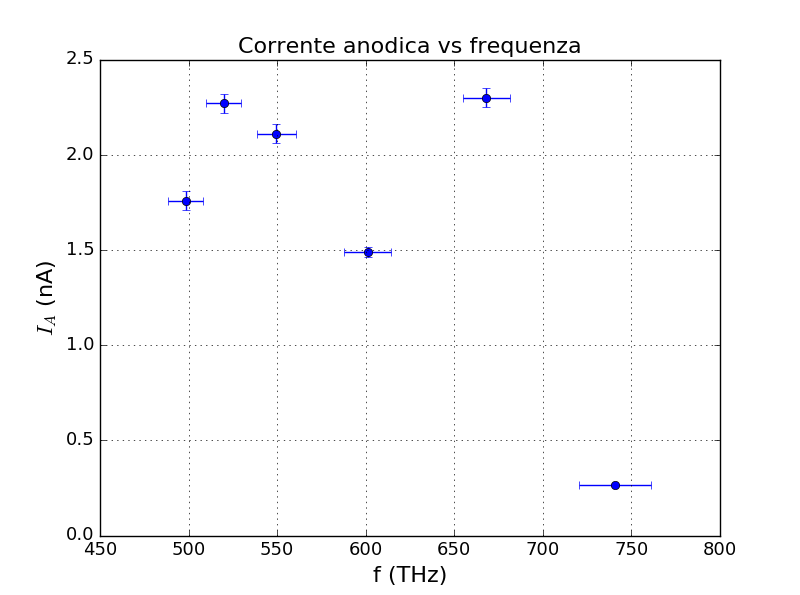
\includegraphics[scale=0.7]{correnteanodica.png}
\caption{Valori della corrente anodica in funzione delle frequenze.\label{fig:correnteanodica}}
\end{figure}
Dal grafico non si riesce ad evincere un andamento particolare della corrente anodica.
Si può osservare che per il filtro blu, la corrente anodica ha un valore decisamente più basso che per gli altri filtri. 

\section{Conclusioni}
Il metodo di fit A (fit con parabola) non ha portato a stime sensate del potenziale di azzeramento.
Il filtro arancione non rispecchia l'andamento per motivi che si possono ricondurre all'apparato sperimentale (struttura del fotomoltiplicatore).
Non abbiamo trovato spiegazioni convincenti per quanto riguarda il comportamento del filtro blu.
La corrente anodica dipende debolmente dal potenziale applicato (sebbene si sia assunto il contrario in fase di fit).

\end{document}


